% --
% game design

\section{Game Design}\label{sec:game_design}
The game design includes essentially all considerations regarding rules, game mechanics, ideas, level and character designs, story and many more. 
Prior to explaining the game and its rules, it is important to mention the game menu and its vital settings for the input microphone device.
The game rules explain the win and loose condition of the video game.
Game mechanics define how the player interacts in the world and how to create actions that change the states of dedicated game objects.
A level design describes and presents the actual levels of the game.

The background story of the game is that a spaceship crashed on a strange planet and the astronaut, named \emph{Jim}, has to find parts of the spaceship in order to repair it.
Strangely, Jim is able to move parts of walls within this world by the use of his voice.


% --
% menu

\subsection{Menu}\label{sec:game_design_menu}
The main menu is the first screen that appears when starting a video game. 
It usually consists of several selectable buttons that are referencing for instance to the start of the actual game, a link to the help menu or the options menu for graphic and music settings of the game.
The main and help menu of the deployed video game is shown in \rfig{game_design_menu_mainhelp}.
\begin{figure}[!ht]
  \centering
  \subfigure[Main Menu]{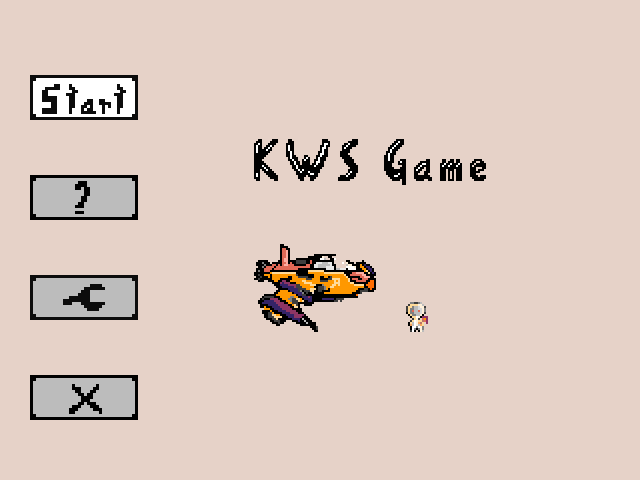
\includegraphics[width=0.45\textwidth]{./6_game/figs/game_design_menu_main.png}}
  \qquad
  \subfigure[Help Menu]{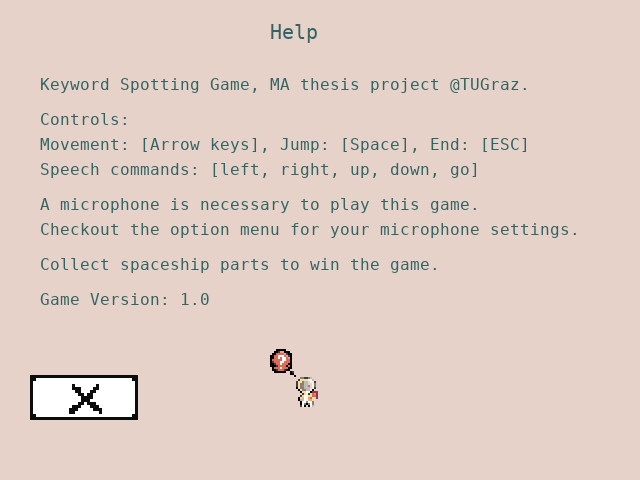
\includegraphics[width=0.45\textwidth]{./6_game/figs/game_design_menu_help.png}}
  \caption{Main and help menu of the KWS game.}
  \label{fig:game_design_menu_mainhelp}
\end{figure}
\FloatBarrier
\noindent
The option menu has to be tailored to fit the requirements of a KWS system.
With speech input deployed in a video game, a screen for the settings of the recording input device is strongly recommended.
All available microphone input devices should be visualized in a list and being selectable in order to switch between the independent devices.
Further a small visualization bar of the input signal energy from the selected device is beneficial, so that the user can verify its correct functionality.
An option for adjusting the energy threshold, by which the online system triggers the onset of a speech command, must be added if this property is used within the video game.
The threshold must be adjustable because of varying recording amplification factors in different microphone set-ups.
Another useful screen in the option menu is the visualization of the class dictionary and the output of the actual KWS system.
This screen writes the identified key word onto the display once the onset detection triggers the beginning of a new key word.
All option menu screens are shown in \rfig{game_design_menu_options}.
\begin{figure}[!ht]
  \centering
  \subfigure[Speech Commands]{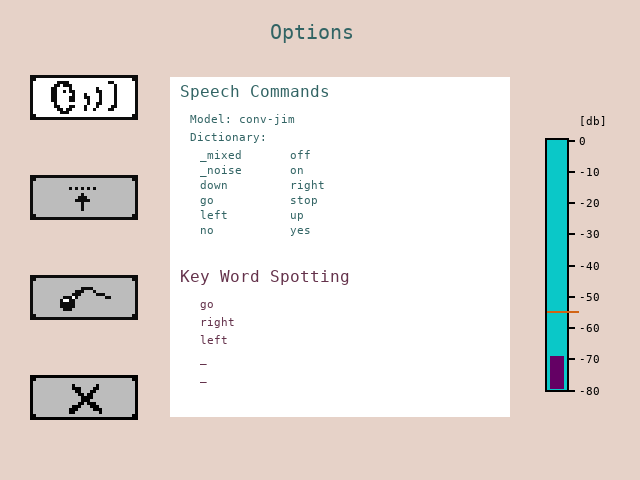
\includegraphics[width=0.45\textwidth]{./6_game/figs/game_design_menu_options_command.png}}
  \qquad
  \subfigure[Threshold]{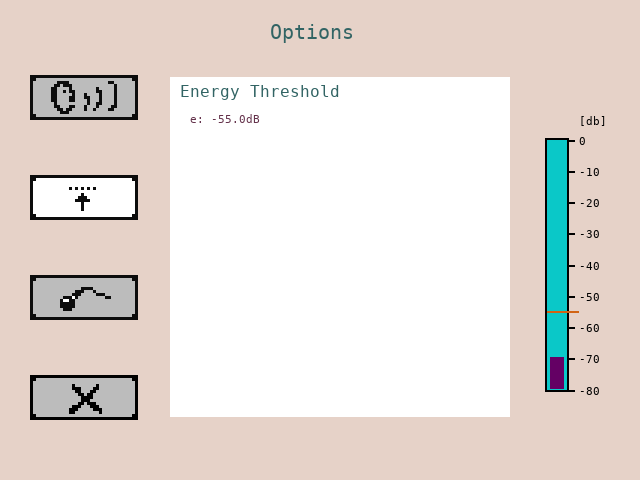
\includegraphics[width=0.45\textwidth]{./6_game/figs/game_design_menu_options_thresh.png}}
  \qquad
  \subfigure[Device]{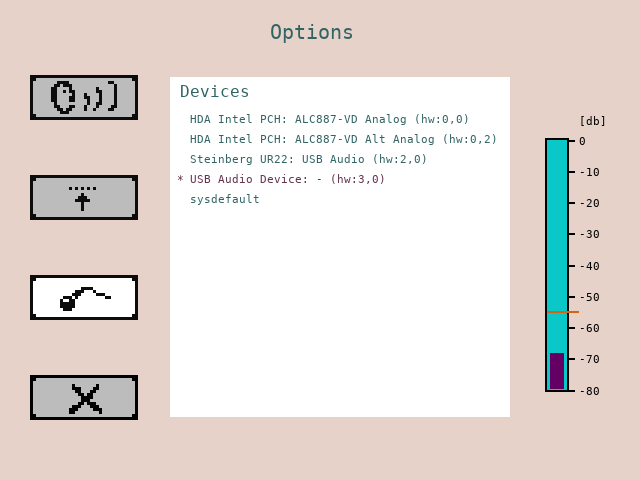
\includegraphics[width=0.45\textwidth]{./6_game/figs/game_design_menu_options_device.png}}
  \caption{Option menu with screens for the input device, the energy threshold, and the KWS system to classify speech commands.}
  \label{fig:game_design_menu_options}
\end{figure}
\FloatBarrier
\noindent


% --
% game rules

\subsection{Game Rules}\label{sec:game_design_rules}
A simple adventure game in a 2D-platformer view (movement are left-right and jump, like the classical \enquote{Super Mario} games) was implemented, where the player has to collect objects and dodge enemies.
The win and loose condition of the game describe the rules to either win or loose the game.
To satisfy the win condition, the player has to collect a single object within each individual level.
Where the levels had been designed such that the player has to use speech commands in order to collect the desired object.
On the other hand to satisfy the loose condition, the player has to collide with an enemy which of course should be avoided.
If the player runs into an enemy, a loose screen appears and the same level has to be restarted from its initial state.


% --
% game mechanics

\subsection{Game Mechanics}\label{sec:game_design_mechanics}
Game mechanics with KWS have to consider time delays because of the processing time speech signals require.
In this thesis the KWS system was used as augmented input control, where the game does not depend entirely on the processing of speech commands as inputs.
The controlling of the character is handled with standard keyboard keys for movement, so that the player receives immediate feedback. 
The speech command control performs a two dimensional grid move upon a so called moveable block, by speaking the command word for the intended direction, as for instance \enquote{left} and \enquote{right} or \enquote{up} and \enquote{down}.
A level can contain several moveable blocks and the switch between those is done by the command word \enquote{go}, until the desired moveable block is selected.
The selected movable block is highlighted with a different color to distinguish it from the other moveable blocks.
Further all movable blocks share the same base color to distinguish them from ordinary walls.
At all times only one of all moveable block can be controlled by the player.
The moveable blocks, walls and the collectable object are shown in \rfig{game_design_mechanic_thing} from a section of Level One.
\begin{figure}[!ht]
  \centering
  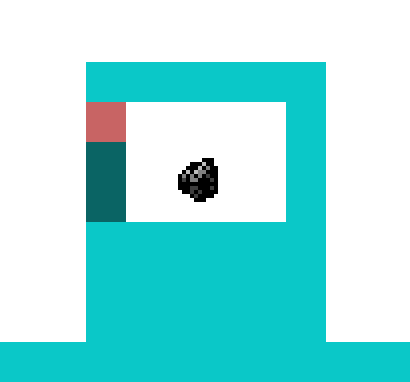
\includegraphics[height=0.25\textwidth]{./6_game/figs/game_design_mechanic_thing.png}
  \caption{A Section of Level One that shows the moveable blocks presented in a darker base color than the usual walls and the active moveable wall highlighted in red.}
  \label{fig:game_design_mechanic_thing}
\end{figure}
\FloatBarrier
\noindent
If a player speaks out a command word that does not correspond to a movement but is included in the class dictionary, as for instance \enquote{yes}, or a command word is spoken that is not in the dictionary, hence it corresponds to the \enquote{\_mixed} label, a small bubble with a question mark is shown next to the player character for a few frames.
The indication of the \enquote{\_noise} label is done similarly but with a bubble that includes a spiral intended as rubbish symbol.
Both bubbles including the player character are shown in \rfig{game_design_mechanic_bubble}.
\begin{figure}[!ht]
  \centering
  \subfigure[\enquote{\_mixed} label]{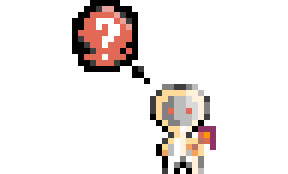
\includegraphics[height=0.13\textwidth]{./6_game/figs/game_design_mechanic_bubble_question.png}}
  \hspace{2 cm}
  \subfigure[\enquote{\_noise} label]{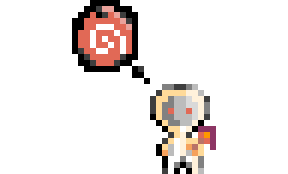
\includegraphics[height=0.13\textwidth]{./6_game/figs/game_design_mechanic_bubble_rubbish.png}}
  \caption{Handling of the \enquote{\_mixed} and \enquote{\_noise} label by displaying bubbles next to the player character.}
  \label{fig:game_design_mechanic_bubble}
\end{figure}
\FloatBarrier
\noindent
In order to provide a loose condition within the game, as already mentioned in \rsec{game_design_rules}, enemies were implemented.
The player can perform jumps to dodge enemies.
The enemies move from left to right and change their direction when an obstacle like a wall is hit.
The enemy sprite sheet is shown in \rfig{game_design_mechanic_enemy}.
\begin{figure}[!ht]
  \centering
  
\includegraphics[height=0.07\textwidth]{./6_game/figs/game_design_mechanic_enemy.png}
  \caption{Enemy sprite sheet.}
  \label{fig:game_design_mechanic_enemy}
\end{figure}
\FloatBarrier
\noindent


% --
% level design

\subsection{Level Design}\label{sec:game_design_level}
Two levels that use the game mechanic of movable blocks, as described previously in \rsec{game_design_mechanics}, were implemented.
The first level introduces the player to the game.
The player learns how the game mechanics work and how to command the moveable blocks out of the path to the collectable object.
In the second level the player has to align the moveable blocks, such that by jumping upon them, higher plateaus can be reached.
The levels are both shown in \rfig{game_design_level}.
\begin{figure}[!ht]
  \centering
  \subfigure[Level One]{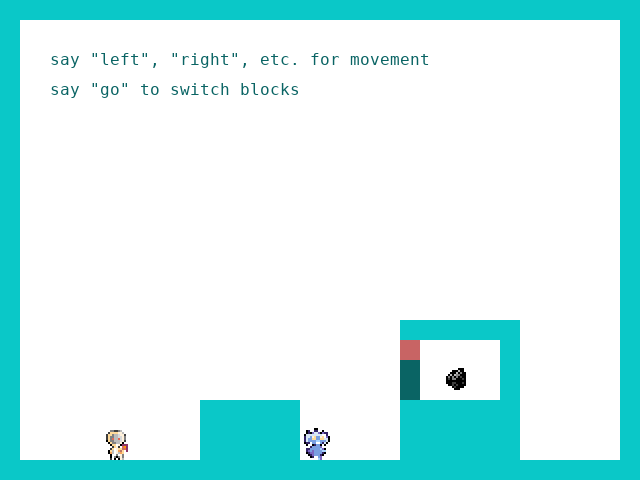
\includegraphics[width=0.45\textwidth]{./6_game/figs/game_design_level_one_start.png}}
  \qquad
  \subfigure[Level Two]{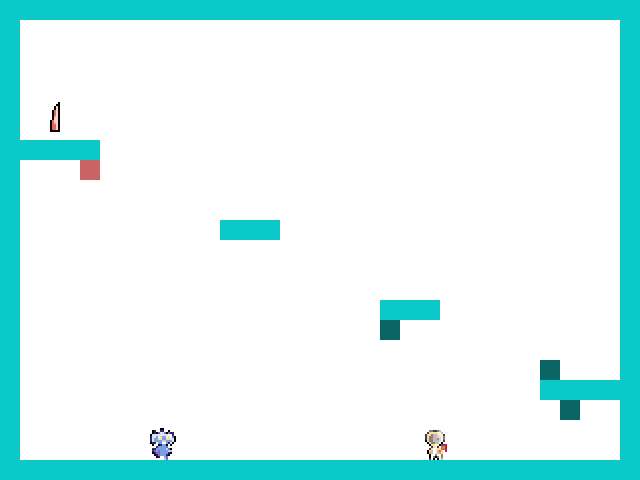
\includegraphics[width=0.45\textwidth]{./6_game/figs/game_design_level_two_start.png}}
  \caption{Level design of the implemented levels.}
  \label{fig:game_design_level}
\end{figure}
\FloatBarrier
\noindent
The completion of a level is done by collecting one part of the spaceship that is placed in the level.
A screen that shows the spaceship plus the collected spaceship part appears and the player has to press enter to continue to the next level.
If the player collides with an enemy, a simple loosing screen appears and the player has to retry the same level.
Both scenarios with both complete and loose screen of Level One is shown in \rfig{game_design_level_complete}.
\begin{figure}[!ht]
  \centering
  \subfigure[Level One Complete]{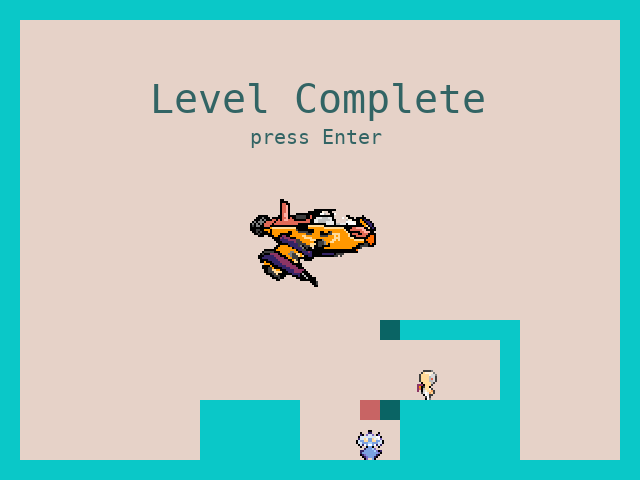
\includegraphics[width=0.45\textwidth]{./6_game/figs/game_design_level_one_complete.png}}
  \qquad
  \subfigure[Level One Loose]{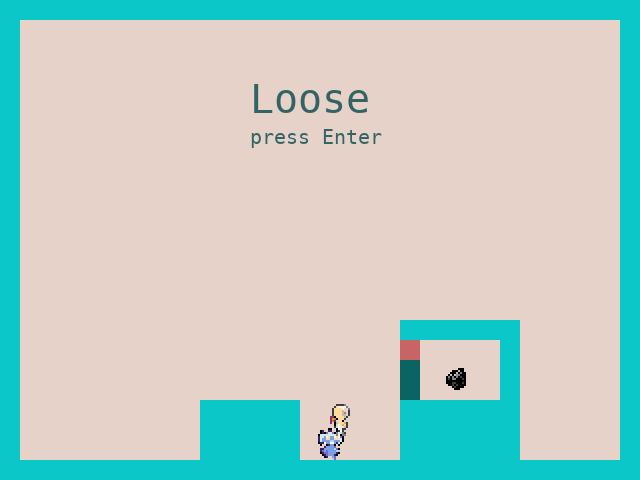
\includegraphics[width=0.45\textwidth]{./6_game/figs/game_design_level_one_loose.png}}
  \caption{Completing and loosing Level One.}
  \label{fig:game_design_level_complete}
\end{figure}
\FloatBarrier
\noindent